\documentclass[10pt]{article}

\newcommand{\boldit}[1]{\textbf{\textit{#1}}}
\usepackage{xcolor}
\usepackage{graphicx}
\usepackage{tikz}
\usetikzlibrary{mindmap}

\begin{document}

\section{\textsf{Introduction}}
\boldit{testing something}

image 1 
\begin{figure}[hbt!]
  \centering
  
\includegraphics{usyd}
\end{figure}

Logo of The University of Sydney \footnote{image from Google}

Testing attempt 1
\begin{itemize}
  \item Amy Push attempt 1
  \item Adam attempt to test 1
  \item New item added
\end{itemize}
New line written

\textcolor{red}{New line} by the branch master

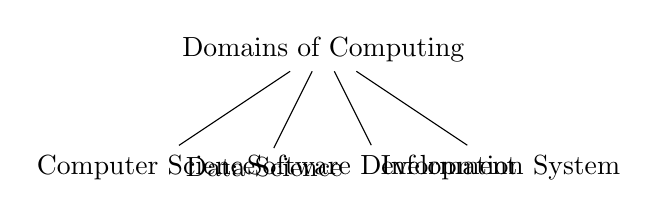
\begin{tikzpicture}
\node{Domains of Computing}
     child { node {Computer Science} }
     child { node {Data Science} }
     child { node {Software Development} }
     child { node {Information System} }
;
\end{tikzpicture}

A line written by the new branch

New attempt by Amy


Trying for automatic merge
second test

SomeThing new
\end{document}
